\chapter{Progetto}

\section{Architettura}
La soluzione proposta si avvale di una architettura ibrida, che prova a conciliare le i servizi e le opportunità
che l'utilizzo della blockchain offre con le sue limitazioni intrinseche. \\
Invece che provare ad abbracciare a tutti i costi un modello esclusivamente distribuito, si è optato per
mantenere un approccio più tradizionale per quanto riguarda l'immagazzinamento e la gestione dei dati. \\

Si individuano quindi i seguenti agenti (\autoref{lab:did-architecture}):
\begin{itemize}
    \item un numero arbitrario di \gls{der} che fa capo ad un \gls{prosumer}
    \item un numero arbitrario di \gls{prosumer} che fa capo ad un \gls{aggregator}
    \item un \gls{aggregator}
    \item una DApp, che rappresenta un interfaccia per per consultare i dati
\end{itemize}

\begin{figure}[h]
    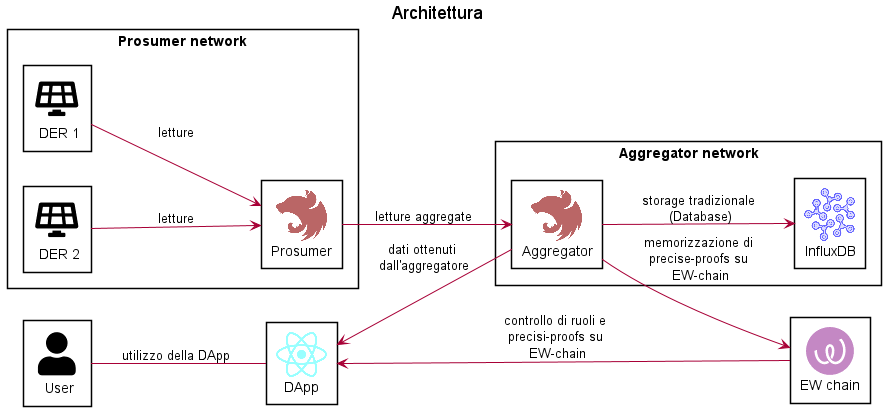
\includegraphics[width=\linewidth,keepaspectratio]{diagram-architecture.png}
    \centering
    \caption{Un esempio di architettura che include un \gls{prosumer} che possiede due \gls{der} ed un \gls{aggregator}}
    \label{lab:diagram-architecture}
\end{figure}

Al \gls{prosumer} si assegna un ruolo di rilievo, in quanto responsabile per la creazione delle precise-proof
che garantiscono l'integrità e il non ripudio dei dati. \\
\\
All'\gls{aggregator} spetterà il compito di verificare la correttezza e la validità dei dati acquisiti,
sfruttando varie tecnologie crittografiche e i servizi offerti da \gls{ew}.
Se la validazione va a buon fine, i dati vengono salvati su un database tradizionale. \\
Contemporaneamente viene eseguito un apposito metodo sullo smart contract designato nella blockchain,
che emetterà un log con il DID dell'\gls{aggregator} e la precise-proof associata alle letture. (\autoref{lab:diagram-flow-aggregator})\\

\begin{figure}[H]
    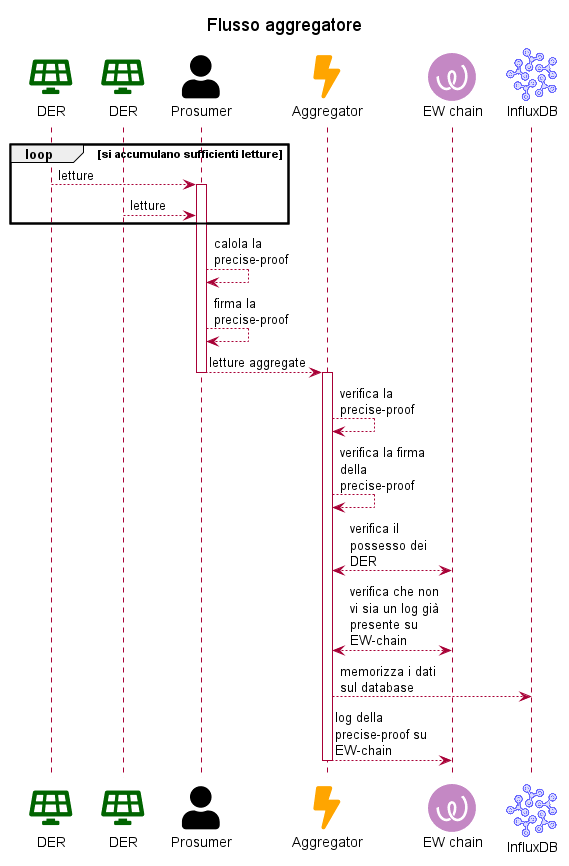
\includegraphics[scale=0.5]{diagram-flow-aggregator.png}
    \centering
    \caption{Diagramma di sequenza che rappresenta il flusso per la registrazione di nuove letture}
    \label{lab:diagram-flow-aggregator}
\end{figure}

Una possibile interfaccia, realizzata tramite DApp, può sfruttare il sistema di \gls{iam} offerto da \gls{ew}
per consentire l'accesso e la visualizzazione dei dati richiedendo un'autenticazione minimale,
che viene delegata alla crittografia asimmetrica usata tradizionalmente sulle blockchain (\autoref{lab:diagram-flow-dapp}). \\


\begin{figure}[H]
    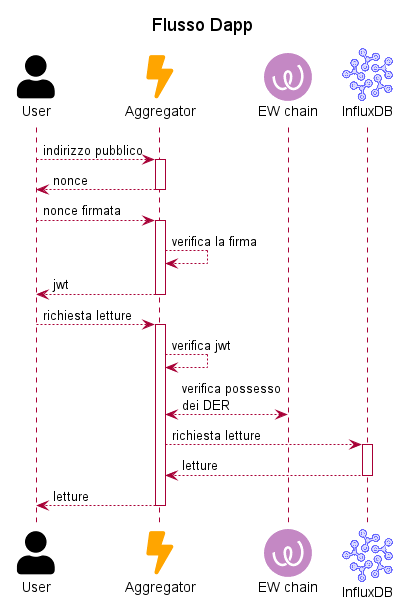
\includegraphics[scale=0.5]{diagram-flow-dapp.png}
    \centering
    \caption{Diagramma di sequenza che rappresenta il flusso per la lettura di dati dall'\gls{aggregator}}
    \label{lab:diagram-flow-dapp}
\end{figure}


\section{Componenti}

\subsection{DER}
I protagonisti del progetto sono proprio i DER, in una visione che li vuole identificare come dispositivi \gls{iot} piuttosto semplici.
L'unico requisito che devono soddisfare i DER è di avere una connessione alla rete locale per poter utilizzare il protocollo \gls{http}. \\
Le letture possono essere effettuate ad una cadenza arbitraria stabilita dall'\gls{oem} o dall'ente competente che ha installato il dispositivo. \\
Il dispositivo ha volutamente un ruolo molto limitato. Non è necessario che sia a collegato con altri \gls{der}
o che possieda ulteriori informazioni oltre quelle prodotte dal suo funzionamento e il \gls{did} che lo identifica. \\
L'unica comunicazione che il dispositivo effettua tramite la rete locale è verso l'applicazione del \gls{prosumer}.
Non è necessario sia connesso alla rete internet perché il protocollo funzioni. \\
Il payload (\autoref{lab:der-payload}) inviato è estremamente semplice e contiene solo le informazioni essenziali,
quali il \gls{did} del dispositivo, il timestamp e il valore registrato con la lettura, compresa l'unità di misura. \\

\begin{listing}
    \begin{minted}{json}
{
    "assetDID": "did:ethr:0x0000000000000000000000000000000000000000",
    "timestamp": "2020-01-01T00:00:00Z",
    "value": 100,
    "unit": "Wh"
}
\end{minted}
    \caption{Esempio di payload mandato dal \gls{der} all'\gls{prosumer}}\label{lab:der-payload}
\end{listing}

Il \gls{der} può essere simulato con l'invio periodico dei dati al \gls{prosumer} locale tramite uno script come questo:
\inputminted[linenos]{bash}{../der/iot_source.sh}

\subsection{Prosumer}
Il \gls{prosumer} in questo contesto si riferisce ad un'applicativo che ha il compito
di mettere insieme le letture provenienti da più \gls{der} della \gls{lan} a cui appartiene. \\
Il \gls{prosumer} è una applicazione web che espone una semplice \gls{api} \gls{rest} attraverso la quale ricevere le letture accumulandole. \\
Dopo aver raggiunto un numero sufficiente di letture, che in questo caso sono banalmente memorizzate in un database
SQLite\cite{sftw:sqlite}, il \gls{prosumer} crea una precise-proof che le vincola. \\
Il vantaggio di usare una precise-proof basata sulla radice di un albero di Merkle (cfr. \autoref{sec:merkle-tree}) è che,
qualora fosse necessario dimostrare di aver effettuato e comunicato correttamente una lettura specifica all'\gls{aggregator},
sarà sufficiente mostrare il singolo dato incriminato e fornire gli hash dei nodi adiacenti necessari a ricostruire l'albero,
riducendo in modo significativo la quantità di dati potenzialmente sensibili da condividere. \\
Il \gls{prosumer} firmerà poi con la sua chiave privata la precise-proof. \\
Ciò fornisce all'\gls{aggregator} una garanzia sul proprio interlocutore e protegge la precise-proof, e di riflesso l'intero payload,
da possibili alterazioni. \\
Viene quindi costruito un payload (\autoref{lab:prosumer-payload}) che contiene la lista di tutti i dati e il valore della precise-proof.
A ciò si aggiunge la lista dei valori di salt utilizzati nella creazione dell'albero e la firma digitale applicata alla precise-proof, oltre che informazioni di comodità
come i timestamp della prima e ultima lettura. \\
Dopo aver mandato il proprio payload, interfacciandosi direttamente con la \gls{ewc} è possibile captare i log prodotti dallo smart contract di riferimento
che contengono la precise-proof contenuta nel payload.
Una volta ricevuto il log, si ha la garanzia che tutto il flusso è andato a buon fine e che la precise-proof rimarrà perennemente registrata e consultabile.

\begin{listing}[h]
    \begin{minted}{json}
{
    "start": "2022-01-01T00:00:00Z",
    "stop": "2022-01-02T00:00:00Z",
    "rootHash": "09urv0un981evup2m8u3",
    "salts": [
        "salt1",
        "salt2"
    ],
    "status": "NotSubmitted",
    "readings": [
        {
            "assetDID": "did:ethr:0x0000000000000000000000000000000000000000",
            "timestamp": "2022-01-01T00:00:00Z",
            "value": 10000000,
            "unit": "Wh"
        },
        {
            "assetDID": "did:ethr:0x0000000000000000000000000000000000000000",
            "timestamp": "2022-01-02T00:00:00Z",
            "value": 1000,
            "unit": "Wh"
        }
    ],
    "signature": "signed root hash"
}
\end{minted}
    \caption{Esempio di payload mandato dal \gls{prosumer} all'\gls{aggregator}}\label{lab:prosumer-payload}
\end{listing}

\subsection{Aggregator}
L'\gls{aggregator} offre un servizio pubblico a cui i \gls{prosumer} della sua giurisdizione fanno riferimento.
Il suo ruolo è principalmente di controllo, e si limita a raccogliere i dati che riceve, verificare che siano corretti e
assicurarsi che il mittente sia autorizzato a compiere questa azione. \\
Ciò viene fatto in un primo luogo verificando la firma digitale della precise-proof.
Successivamente viene ricostruito l'albero di Merkle a partire dalle letture e dai salt e si verifica che la precise-proof corrisponda.
Per finire, viene consultata la \gls{ewc} per controllare che il mittente sia anche il proprietario di tutti i \glsplural{der} che figurano nelle letture. \\
Se tutti questi controlli sono andati a buon fine, le informazioni sono salvate in un database InfluxDB \cite{sftw:influxdb}, specializzato nell'immagazzinamento di dati sotto forma di serie storiche.
Infine viene chiamato il metodo il metodo \textbf{store} sullo smart contract \textbf{ReadingsNotary} (\autoref{lab:readings-notary}), attualmente presente su Volta all'indirizzo \href{https://volta-explorer.energyweb.org/address/0xe574fDD8C3148f2E883612A9C6CDA7b9C12d1566/transactions}{0xe574fdd8c3148f2e883612a9c6cda7b9c12d1566}.

\begin{listing}[h]
    \begin{minted}{solidity}
// SPDX-License-Identifier: MIT
pragma solidity 0.8.4;

contract ReadingsNotary {
    /** A new metered reading has been emitted */
    event NewMeterReading(address indexed operator, bytes indexed proof);

    /** Store a new reding
     * @param _proof Merkle root of the tree of merkle proofs of the aggregated readings
     */
    function store(bytes calldata _proof) external {
        emit NewMeterReading(msg.sender, _proof);
    }
}
\end{minted}
    \caption{Smart contract \textbf{ReadingsNotary}, rilasciato su Volta all'indirizzo \textit{0xe574fdd8c3148f2e883612a9c6cda7b9c12d1566}}\label{lab:readings-notary}
\end{listing}

L'\gls{aggregator} fornisce pubblicamente una interfaccia \gls{api} \gls{rest} che consente di accedere ai dati memorizzati al fine di consultarli.
L'accesso è protetto da un sistema di autenticazione che si svolge in due fasi:
\begin{itemize}
    \item si richiede una nonce generata sul momento dal \gls{aggregator} associandola alla propria chiave pubblica
    \item si invia la firma digitale della nonce al passaggio precedente, ottenendo un \gls{jwt} con validità di 24 ore dall'\gls{aggregator}
\end{itemize}

Un utente ha accesso solo ai dati relativi ai \gls{did} che possiede.
Fa eccezione l'utente \gls{aggregator}, che può accedere a tutti i dati memorizzati nel database.

\subsection{DApp}
Il \gls{dapp} è una applicazione web che consente di accedere ai dati memorizzati dall'\gls{aggregator}.
Il login viene effettuato tramite Metamask (cfr. \autoref{sec:metamask}).
Si ha quindi la possibilità di firmare la nonce per autenticarsi con il server dell'\gls{aggregator}. \\
Una volta effettuato l'accesso, la web app verifica automaticamente i claim associati ad \gls{did} dell'utente
che ha eseguito il login, e se verifica che è presente il ruolo di \gls{prosumer}, viene visualizzata l'interfaccia apposita.
Altrimenti viene visualizzata una pagina con informazioni meno dettagliate. \\
Da questa interfaccia è possibile consultare i dati memorizzati dal prosumer, visualizzati tramite un grafico.

% TODO: add a screenshot of the DApp

\section{Implementazione}

\subsection{\gls{bom}}
Al fine di realizzare tutte le componenti di questa architettura sono state utilizzate le seguenti librerie, framework e tecnologie:

\begin{itemize}
    \item \textbf{SQLite} \cite{sftw:sqlite}: implementazione di un SQL database engine piccolo, veloce ed affidabile
    \item \textbf{InbluxDB} \cite{sftw:influxdb}: database specializzato per immagazzinare dati sotto forma di serie storiche
    \item \textbf{NestJS} \cite{sftw:nestjs}: framework javascript per la creazione di applicazioni web back-end
    \item \textbf{hardhat} \cite{sftw:hardhat}: framework javascript per la creazione e il deploy di smart contracts su blockchain
    \item \textbf{iam-client-lib} \cite{sftw:iam-client-lib}: libreria javascript realizzata da \gls{ew} usata per interagire con il loro servizio di \gls{iam}
    \item \textbf{react} \cite{sftw:react}: framework javascript per la creazione di applicazioni web
    \item \textbf{ethers} \cite{sftw:ethers}: libreria javascript usata per interfacciarsi con la blockchain
\end{itemize}

\subsection{Setup locale}
Per ottenere una simulazione fedele di più componenti che interagiscono fra loro in un sistema distribuito come quello proposto e
per offrire la possibilità di ricreare l'intera architettura facilmente e senza requisiti complessi, è stato utilizzato il sistema di containerizzazione Docker \cite{sftw:docker}. \\
La repository git contiene un file \textit{docker/docker-compose.yml} utilizzabile per inizializzare tutti i container necessari per l'esecuzione dell'architettura.
Sebbene la maggior parte dei parametri di default sia adatta alla maggior parte dei casi d'uso, vi sono alcuni parametri che è necessario sovrascrivere. \\
Poiché si tratta di dati sensibili, è consigliabile creare nella stessa cartella un file \textit{docker/docker-compose.override.yml} (\autoref{lab:docker-compose-override}) contenente i parametri da sovrascrivere,
per evitare di eseguirne il commit in un repository pubblico.

\begin{listing}[H]
    \begin{minted}{yaml}
version: "3.9"

services:
  aggregator:
    environment: # Chiave segreta o mnemonic dell'aggregatore. Assicurarsi di avere a disposizione qualche Volta token
      SK: swear fest avoid yolk cat dog tagging water bag coat wardrobe

  prosumer:
    environment: # Chiave segreta o mnemonic del prosumer
      SK: swear fest avoid yolk cat dog tagging water bag coat wardrobe
\end{minted}
    \caption{Esempio di \textit{docker/docker-compose.override.yml}}\label{lab:docker-compose-override}
\end{listing}

Per avviare l'intero stack, eseguire il comando \mintinline{bash}{$ docker-compose up} nella directory \textit{docker}. \\
Per fermare l'esecuzione, eseguire \mintinline{bash}{$ docker-compose down}. \\
Per rimuovere i volumi Docker rimasti, eseguire \mintinline{bash}{$ docker volume prune}.
